\documentclass{csfourzero}

\title{Latency Performance Comparison of Open Source Real-Time Publish-Subscribe Data Distribution Service Implementations}
\author{Marcel Zak}
\date{\today}
% A useful package to support on-line references
\usepackage{url}
\usepackage{natbib}
\usepackage{graphicx}

\bibliographystyle{plain}
\abstract{I performed an empirical evaluation of latency performance of two popular open source implementations of RTPS DDS protocol. Those two libraries were eProsima Fast RTPS and OpenDDS. The presented results clearly show that eProsima Fast RTPS is two times faster in terms of latency performance than OpenDDS. This was confirmed with both, "Best effort" and "Reliable", transport types.}


\begin{document}
\maketitle

%\tableofcontents
%\newpage 

\section{Introduction}
\label{sec:intro}

\quad In this research paper, I decided to investigate a difference in latency performance in two popular open source implementations of Data Distribution Service (DDS) protocol. DDS is middleware developed by Object Management Group (OMG) \cite{what-is-dds}. It is specifically designed as a machine to machine, data-centric, high performance and reliable protocol. OMG aimed to create a protocol that does not have a problem with scalability and it fulfils requirements for the modern Internet of Things (IoT) applications \cite{DDS-spec}. Later a Real-Time Publish-Subscribe (RTPS) DDS was specified (by OMG) as the interoperability protocol. RTPS DDS was designed as real-time, low latency protocol for best effort and reliable communication over unreliable transports such as UDP/IP and it is standardized that different RTPS implementations can communicate with each other \cite{RTPS-spec}. For its quality and robustness, it is often used in aerospace and defence sectors for real-time applications \cite{eprosima-rtps-intro}. 

For real-time applications, delivering the right message at the right time to the right place is critical. Such systems are widely used in automation, robotics, space industry, medicine and other sectors. Time and reliability are the most important factors in these systems. Therefore, the right choice of a library is crucial. 

These two open source libraries implement the same RTPS protocol specification. They are implemented in C++. The first implementation is OpenDDS \cite{git-openDDS} created by OCI that is a full implementation of DDS. The second library was developed by eProsima and it is standalone RTPS implementation called Fast RTPS \cite{git-eProsima}. It claims to be the fastest one because it is lightweight \cite{eprosima-rtps-intro}. In this paper, I will investigate latency performance of both open source RTPS implementations.

\section{Background and related work}
\label{sec:lit}

\quad Firstly, I describe the underlying design principle behind DDS protocol. Participants (applications) using DDS can publish or subscribe to a specific "topic" of information. A topic is a name that refers to a specific piece of information we want to share. It also contains the definition of Data we want to share \cite{eprosima-dds}. A single participant can publish and subscribe to multiple "topics" at the same time. The advantage of DDS is implementing richer set of Quality of Service parameters \cite{what-is-dds}. It is possible to set up different aspects of the communication. Be it persistence, reliability, redundancy, transport settings, lifespan and many others. The communication model is straightforward. See Figure \ref{fig:GlobalDataSpace}.

\begin{figure}[h]
	\centering
	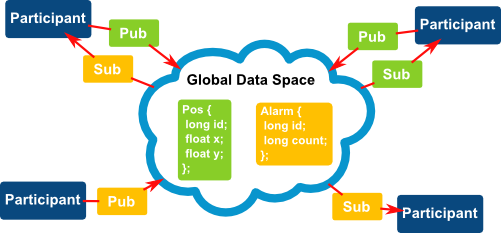
\includegraphics[width=0.6\textwidth]{GlobalDataSpace}
	\caption{\label{fig:GlobalDataSpace}DDS Model: The Global Data Space \cite{eprosima-dds}}
\end{figure}

DDS provides a simple modular design that is shown in Figure \ref{fig:DDSArch}. In these two open source implementations is DDS only a library that is linked to an application. There is no need to install any service or daemon. It is important to note that RTPS is on top of the transport layer in the OSI model. Therefore, DDS can be implemented over any kind of underlying transport \cite{eprosima-dds}. DDS specification does not outline how the message should be delivered. Therefore, multiple implementations exist.

\begin{figure}[h]
	\centering
	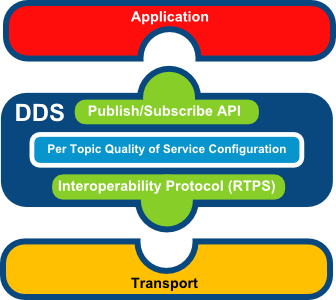
\includegraphics[width=0.5\textwidth]{DDSArch}
	\caption{\label{fig:DDSArch}DDS Architecture \cite{eprosima-dds}}
\end{figure}

Scientific community lacks papers about DDS benchmarking. However, there are two papers worth mentioning. The first one is \textit{Performance assessment of OMG compliant data distribution middleware} \cite{omg-perf}. It discusses the complexity of benchmarking different DDS implementations. In the second paper \textit{Data Distribution Service (DDS): A performance comparison of OpenSplice and RTI implementations} \cite{splice-vs-rti} describes throughput, latency and CPU load comparison of OpenSplice and RTI DDS implementations.

Authors of the first paper decided to develop a tool called DDSBench that should provide a framework for objective performance comparison of different DDS implementations. DDSBench offers a variety of possible settings such as message type, size, publication period, message iteration, QoS and many others. The idea is that a developer models the test environment based on requirements of the specific application and runs the test. Results of the test show which DDS implementation is suitable for the application. It is also discusses different methods for latency measurement. The standard method is \textit{Round-Trip time}. It is the time elapsed between sending a message and receiving it back. However, they decided to use \textit{One-way Transit Time} that represents time elapsed between sending the message from publisher to subscriber. The advantage is that it more accurately represents the elapsed time from subscriber's point of view. On the other hand, there is disadvantage and difficulty involved with precise clock synchronization on both machines  \cite{omg-perf}. I disagree that for the purpose of benchmarking it is necessary to use \textit{One-way Transit Time}. Based on the related literature \textit{Round-Trip time} reveals the difference in implementations \cite{perf-embedded}. At the end, DDSBench is used to evaluate two implementations. The first one is RTI DDS and OpenDDS \cite{omg-perf}. The results clearly show that the RTI has better performance in all dimensions. I tried to use DDSBench with the newer versions of OpenDDS. Unfortunately, I did not manage to run it because the last update of DDSBench was in 2007.

At the beginning of the second paper, the DDS standard is well described. The next part focuses on metrics and measurement techniques. Authors decided to measure five different parameters to completely evaluate the performance differences of OpenSplice and RTI. The measured parameters are \textit{Samples per second, Throughput, Round-Trip time, CPU and Memory usage}. Authors also mentioned that this measurement of latency is widely accepted \cite{perf-embedded}. At the end, they performed benchmarking and the results revealed that OpenSplice performs significantly better than RTI in throughput tests and samples per second, but only with messages of smaller size (up to 2048 bytes). If the size of the messages is higher then RTI performs much better. OpenSplice utilizes federated architecture \cite{federated-arch} and by default uses batching optimization which enables better performance for small size data exchange. On the other hand, decentralized models (no need for separate daemon), such as RTI, do not have a single point of failure or latency issue, unlike OpenSplice. They are also more suitable for large size data exchange \cite{splice-vs-rti}.

\section{Research question}
\label{sec:rq}

\quad It has been shown that DDS implementations differ in performance despite using the same communication standard RTPS. The research papers mentioned above always compared proprietary with open source or partially open source implementation of DDS RTPS protocol. But when a developer has to choose between open source implementations, to the best of my knowledge there has never been done any performance comparison. Latency is one of the most important factors in critical real-time applications. Therefore, I decided to investigate latency performance of OpenDDS \cite{git-openDDS} and eProsima Fast RTPS \cite{git-eProsima}. 

I chose these two implementations for their popularity and still active development. OpenDDS uses federated model meanwhile Fast RTPS uses fully distributed model. As described in the previous section, each has its advantages and disadvantages. It is not possible to only look at performance tests of both implementations shown on their web pages because these tests were not done in the same testing environment \cite{eProsima-perf, openDDS-perf}. Therefore, the latency times vary and cannot be directly compared.

The research questions are as follows:
\begin{itemize}
	\item Does federated model of OpenDDS introduces latency overhead in comparison to fully distributed model of Fast RTPS?
	\item How does the size of a message influence latency time in federated model vs fully distributed one?
	\item Which one should be chosen if the latency performance is the most important factor?
\end{itemize}

In order to answer these questions, I conduct an experiment that measures the latency of both implementations. I use several standard message sizes to evaluate the behavior in different scenarios. For the purpose of measurement latency, I utilize already implemented performance tests in both libraries. They are using \textit{Round-Trip time} measurement for estimation of latency.

\section{Experimental Design}
\label{sec:exp}

\quad These are my hypotheses:
\begin{itemize}
	\item H0: There will be no difference in latency performance between eProsima Fast RTPS and OpenDDS, regarding all tested message sizes.
	\item H1: There will be the difference in latency performance between eProsima Fast RTPS and OpenDDS, regarding all tested message sizes.
	\item H2: There will be the difference in latency performance between eProsima Fast RTPS and OpenDDS, but only in some tested message sizes.
\end{itemize}

I will measure the latency using loopback interface from the start of send to end of the read. It is the same concept as if I had two separate hosts. In this scenario host1 = host2. See Figure \ref{fig:test-topology}

\begin{figure}[!h]
	\centering
	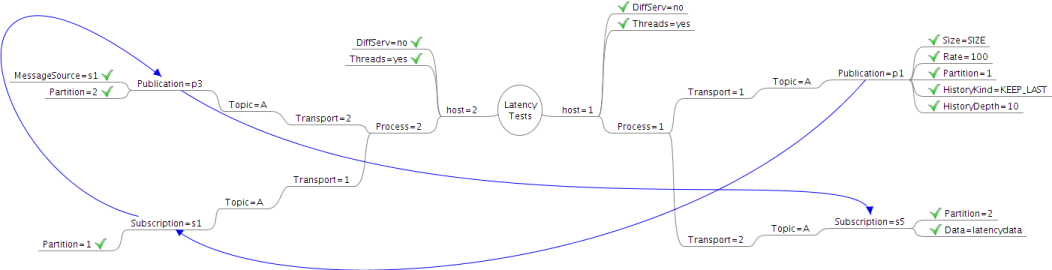
\includegraphics[width=1\textwidth]{openDDS-latency-tests}
	\caption{\label{fig:test-topology}Latency test topology
	\cite{openDDS-test-topology}}
\end{figure}

For this experiment I used one laptop HP EliteBook 2540p with the following parameters: 

\begin{itemize}
	\item CPU: Intel(R) Core(TM) i5 CPU M 540 locked at 1.2GHz frequency
	\item Memory: SAMSUNG 8GB 2x4GB PC3-10600 DDR3 1333MHZ
	\item Operating System: Fedora 27 64-bit
	\item VM Swappiness: 0
	\item Used compiler: gcc version 7.2.1 20170915 (Red Hat 7.2.1-2) (GCC)
	\item CMake: version 3.9.6
	\item OpenDDS version 3.12 (commit: 3057ef9dbb032bc51895f70e5c350af4b10093fa) 
	\item eProsima Fast RTPS (commit: bec4a979c088a1f978af3dfdea2a72ae2a78b52a)
\end{itemize}

The dependent variable latency will be measured with \textit{Round-Trip time} and then divided by two. This represents the time between sending and receiving a message from a publisher to a subscriber. I will discard first 1000 samples and then collect next 10 000 measurements of \textit{Round-Trip time} divided by two. This process will repeat for every message size which is the first independent variable. The sizes of a message will be 16, 32, 64, 128, 256, 512, 1024, 2048, 4096, 8192 and 16384 bytes. The second independent variable is transport type. I will collect data for both "Reliable" and "Best effort" transport types. Both use datagram (UDP/IP) but "Reliable" type uses also RTPS ACKs/NACKs.

After all data is collected, I will calculate the mean, max, min and standard deviation from 10 000 samples for every message size and transport type. Then I also perform T-tests that should reveal if there is any statistical difference in latency performance of those two libraries.

\section{Results}
\label{sec:results}

\quad Figure \ref{fig:graph-results-comparison} shows the mean latency of each message size calculated from 10 000 samples. It is possible to see the latency difference for both types of transport. The latency increase with "Reliable" transport type for Fast RTPS was on average by 50 microseconds. For OpenDDS the latency increase with "Reliable" transport type was in average by 70 microseconds. The differences in latency performance between those two implementations are enormous.

\begin{figure}[!h]
	\centering
	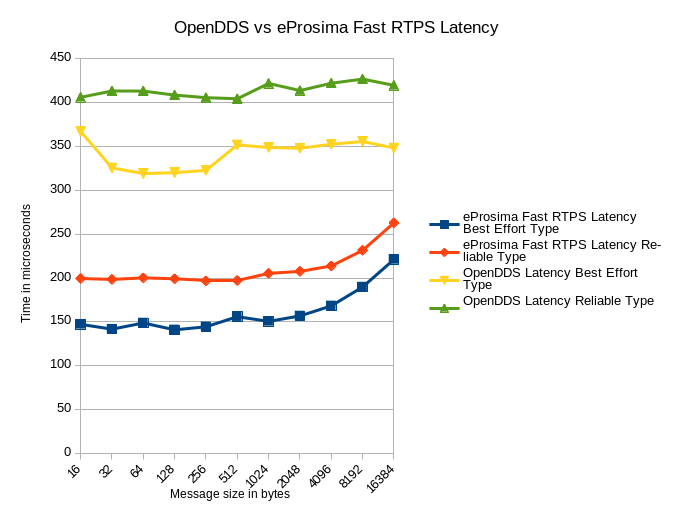
\includegraphics[width=1\textwidth]{graph-results-comparison}
	\caption{\label{fig:graph-results-comparison}OpenDDS vs Fast RTPS Mean Latency of 10 000 samples}
\end{figure}

The Table \ref{eProima-latency-table-best} shows MIN, MAX, MEAN and standard deviation of collected data samples for eProsima Fast RTPS implementation with "Best effort" transport type. We can see on standard deviation values of the measured latency time is very stable. It also slowly increases with bigger message size.

\begin{table}[!ht]
	\centering
	\caption{eProsima Fast RTPS Latency Best Effort Type}
	\label{eProima-latency-table-best}
	\begin{tabular}{|c|c|c|c|c|}
		\hline 
		Message Size (bytes)& MIN & MAX & MEAN & STDEV \\ 
		\hline 
		16 & 113 & 679 & 147.24 & 28.46 \\ 
		\hline 
		32 & 109 & 395 & 141.76 & 23.29 \\ 
		\hline 
		64 & 104 & 622 & 148.82 & 28.08 \\ 
		\hline 
		128 & 108 & 458 & 140.99 & 24.71 \\ 
		\hline 
		256 & 107 & 1 014 & 144.49 & 27.87 \\ 
		\hline 
		512 & 113 & 2 125 & 156.00 & 46.15 \\ 
		\hline 
		1024 & 110 & 615 & 150.62 & 29.53 \\ 
		\hline 
		2048 & 119 & 1 011 & 156.85 & 29.58 \\ 
		\hline 
		4096 & 127 & 894 & 168.33 & 29.42 \\ 
		\hline 
		8192 & 141 & 1 650 & 189.87 & 35.74 \\ 
		\hline 
		16384 & 171 & 2 250 & 221.26 & 45.88 \\ 
		\hline 
	\end{tabular}
\end{table}

The Table \ref{openDDS-latency-table-best} shows the results for OpenDDS implementation. It is evident that the latency values are higher. What is more interesting is that the measured time does not significantly increase even bigger message sizes. It behaves more linearly than in the case of Fast RTPS. It is also interesting that the latency for 16 bytes messages has large standard deviation in comparison to all the others.

\begin{table}[!ht]
	\centering
	\caption{OpenDDS Latency Best Effort Type}
	\label{openDDS-latency-table-best}
	\begin{tabular}{|c|c|c|c|c|}
		\hline 
		Message Size (bytes)& MIN & MAX & MEAN & STDEV \\ 
		\hline 
		16 & 268 & 20 591 & 367.18 & 750.83 \\ 
		\hline 
		32 & 274 & 970 & 325.69 & 29.29 \\ 
		\hline 
		64 & 265 & 476 & 319.18 & 17.95 \\ 
		\hline 
		128 & 265 & 1 034 & 320.24 & 23.51 \\ 
		\hline 
		256 & 267 & 1 408 & 322.91 & 30.18 \\ 
		\hline 
		512 & 256 & 10 408 & 351.89 & 125.48 \\ 
		\hline 
		1024 & 255 & 1 028 & 348.96 & 43.92 \\ 
		\hline 
		2048 & 254 & 1 645 & 348.01 & 47.02 \\ 
		\hline 
		4096 & 264 & 973 & 352.68 & 42.37 \\ 
		\hline 
		8192 & 265 & 875 & 355.75 & 36.90 \\ 
		\hline 
		16384 & 272 & 1 629 & 348.42 & 61.37 \\ 
		\hline 
	\end{tabular}
\end{table}

The Table \ref{T-test-latency-table-best} shows T-test results for every message size for "Best effort" transport type. Based on this we can definitely say that the acquired results are statistically significant. The reason for this is that the p-value is always less than 2.2e-16.

\begin{table}[!ht]
	\centering
	\caption{T-test eProsima vs OpenDDS Latency Best Effort Type}
	\label{T-test-latency-table-best}
	\begin{tabular}{|c|c|c|c|}
		\hline 
		 Message size (bytes) & t & df & p-value \\ 
		\hline 
		16 & -29.271 & 10 028 & \textless 2.2e-16 \\ 
		\hline 
		32 & -490.67 & 19 069 & \textless 2.2e-16 \\ 
		\hline 
		64 & -511.13 & 17 000 & \textless 2.2e-16 \\ 
		\hline 
		128 & -525.5 & 19 949 & \textless 2.2e-16 \\ 
		\hline 
		256 & -434.33 & 19 873 & \textless 2.2e-16 \\ 
		\hline 
		512 & -146.53 & 12 656 & \textless 2.2e-16 \\ 
		\hline 
		1024 & -374.77 & 17 503 & \textless 2.2e-16 \\ 
		\hline 
		2048 & -344.13 & 16 842 & \textless 2.2e-16 \\ 
		\hline 
		4096 & -357.38 & 17 821 & \textless 2.2e-16 \\ 
		\hline 
		8192 & -322.86 & 19 977 & \textless 2.2e-16 \\ 
		\hline 
		16384 & -165.94 & 18 516 & \textless 2.2e-16 \\ 
		\hline 
	\end{tabular} 
\end{table}

The table \ref{eProima-latency-table-reliable} shows significant increase in latency if "Reliable" transport type is used. Also, it is possible to see that the behavior of latency does not change in comparison to "Best effort" transport type.

\begin{table}[!ht]
	\centering
	\caption{eProsima Fast RTPS Latency Reliable Type}
	\label{eProima-latency-table-reliable}
	\begin{tabular}{|c|c|c|c|c|}
		\hline 
		Message Size (bytes)& MIN & MAX & MEAN & STDEV \\ 
		\hline 
		16 & 156 & 6 003 & 199.50 & 97.17 \\ 
		\hline 
		32 & 158 & 6 278 & 198.47 & 81.67 \\ 
		\hline 
		64 & 153 & 1 879 & 200.24 & 29.60 \\ 
		\hline 
		128 & 162 & 2 111 & 199.21 & 31.27 \\ 
		\hline 
		256 & 151 & 2 002 & 196.73 & 29.37 \\ 
		\hline 
		512 & 157 & 1 496 & 197.23 & 26.39 \\ 
		\hline 
		1024 & 160 & 4 892 & 205.35 & 78.35 \\ 
		\hline 
		2048 & 162 & 3 977 & 207.66 & 43.47 \\ 
		\hline 
		4096 & 174 & 796 & 213.82 & 23.38 \\ 
		\hline 
		8192 & 192 & 2 729 & 231.67 & 26.45 \\ 
		\hline 
		16384 & 220 & 1 195 & 262.98 & 28.36 \\ 
		\hline 
	\end{tabular}
\end{table}

In the table \ref{openDDS-latency-table-reliable} are shown the results of latency measurements for OpenDDS with "Reliable" transport type. These results show an increase in latency in comparison to previous transport type. It is also possible to see that standard deviation has significantly increased.

\begin{table}[!ht]
	\centering
	\caption{OpenDDS Latency Reliable Type}
	\label{openDDS-latency-table-reliable}
	\begin{tabular}{|c|c|c|c|c|}
		\hline 
		Message Size (bytes)& MIN & MAX & MEAN & STDEV \\ 
		\hline 
		16 & 320 & 10 696 & 406.19 & 293.54 \\ 
		\hline 
		32 & 326 & 10 585 & 413.39 & 331.99 \\ 
		\hline 
		64 & 322 & 10 611 & 413.24 & 305.65 \\ 
		\hline 
		128 & 322 & 12 149 & 408.68 & 326.76 \\ 
		\hline 
		256 & 324 & 16 763 & 405.78 & 330.79 \\ 
		\hline 
		512 & 306 & 5 333 & 404.52 & 189.25 \\ 
		\hline 
		1024 & 285 & 2 587 & 421.96 & 103.70 \\ 
		\hline 
		2048 & 310 & 7 052 & 413.88 & 212.52 \\ 
		\hline 
		4096 & 316 & 9 462 & 422.22 & 218.54 \\ 
		\hline 
		8192 & 329 & 6 076 & 426.91 & 192.32 \\ 
		\hline 
		16384 & 329 & 5 237 & 419.82 & 91.33 \\ 
		\hline 
	\end{tabular}
\end{table}

The table \ref{T-test-latency-table-reliable} presents T-test results for every message size for "Reliable" transport type. Based on this we can definitely say that the acquired results are statistically significant. The reason for this is that the p-value is always less than 2.2e-16.

\begin{table}[!ht]
	\centering
	\caption{T-test eProsima Fast RTPS vs OpenDDS Latency Reliable Type}
	\label{T-test-latency-table-reliable}
	\begin{tabular}{|c|c|c|c|}
		\hline 
		Message size (bytes) & t & df & p-value \\ 
		\hline 
		16 & -66.85 & 12 164 & \textless 2.2e-16 \\ 
		\hline 
		32 & -62.86 & 11 205 & \textless 2.2e-16 \\ 
		\hline 
		64 & -69.36 & 10 187 & \textless 2.2e-16 \\ 
		\hline 
		128 & -63.79 & 10 182 & \textless 2.2e-16 \\ 
		\hline 
		256 & -62.94 & 10 157 & \textless 2.2e-16 \\ 
		\hline 
		512 & -108.48 & 10 388 & \textless 2.2e-16 \\ 
		\hline 
		1024 & -166.65 & 18 608 & \textless 2.2e-16 \\ 
		\hline 
		2048 & -95.06 & 10 834 & \textless 2.2e-16 \\ 
		\hline 
		4096 & -94.81 & 10 228 & \textless 2.2e-16 \\ 
		\hline 
		8192 & -99.74 & 10 716 & \textless 2.2e-16 \\ 
		\hline 
		16384 & -163.98 & 11 910 & \textless 2.2e-16 \\ 
		\hline 
	\end{tabular} 
\end{table}

Based on the presented results I have to definitely reject the null hypothesis which says that there will be no difference in latency performance between eProsima Fast RTPS and OpenDDS, regarding all tested message sizes. I also have to reject alternative hypothesis number 2 which says There will be the difference in latency performance between eProsima Fast RTPS and OpenDDS, but only in some tested message sizes.

On the other hand, the alternative hypothesis number 1 has been confirmed. It says that there will be the difference in latency performance between eProsima Fast RTPS and OpenDDS, regarding all tested message sizes. It is possible to claim this because all T-tests show p-value less than 2.2e-16.


\section{Discussion}
\label{sec:discuss}

\quad The presented results confirm the hypothesis that there is a difference in latency performance between these two implementations. Based on the presented results I can say that eProsima Fast RTPS is 2 types faster than OpenDDS in terms of latency, regards to all tested message sizes. However, this experiment was performed on a single machine and it would be interesting to do the same experiment on a network with two different physical hosts and compare the results with my experiment. Also, this paper was not focused on the behaviour of latency when the network and devices are approaching saturation point. That means when we would reach the limits of chosen Ethernet network. Such experiment could lead to different results. 

Latency performance is only one of the factors which influence the final decision of a developer which implementation to choose. In a scope of this paper it was the only comparison I have done. It would be interesting to compare these two implementations in terms of throughput, CPU and Memory load and what is the maximum number of messages per second they can deliver. 

\section{Conclusion}
\label{sec:conc}

\quad In this paper, I performed an empirical evaluation of latency performance of two popular open source implementations of RTPS DDS protocol. Those two libraries were eProsima Fast RTPS and OpenDDS. The presented results clearly show that eProsima Fast RTPS is two times faster in terms of latency performance than OpenDDS. This was confirmed with both, "Best effort" and "Reliable", transport types.

\bibliography{myrefs}

\end{document}
